% sesmesh — Solvent Excluded Surface meshes for molecules
% Copyright (c) 2026 Ugo Varetto
% SPDX-License-Identifier: MIT OR Apache-2.0

\section{Performance}
\label{sec:performance}

\paragraph{Machine and protocol.}
All measurements were made on one Apple Silicon machine with 10 cores
(4 performance and 6 efficiency cores) under macOS, with release builds,
all cores and the NEON kernel \todo{state the exact chip, memory size,
macOS and rustc versions}. The machine carried a heavy background load
from other applications during the runs (load average 15--27), so wall
times are pessimistic and repeated runs vary by several percent. The
reference machines of the specification---8 homogeneous performance
cores, and an x86-64 desktop with AVX2---were not available for these runs;
\cref{sec:x86} adds measurements on an idle 16-core x86-64 machine. Peak
memory is the maximum resident set size reported by \code{/usr/bin/time
-l}.

\begin{table}[t]
  \centering
  \caption{Wall time of complete command-line runs (10 cores, loaded
    machine; ranges over repeated runs) from the validation report, with
    the provisional targets of the specification, which were set before
    any measurement and remain goals.}
  \label{tab:perf}
  \small
  \begin{tabular}{@{}llrrrrr@{}}
    \toprule
    Entry & Description & Atoms & $h$ (\AA) & Triangles & Measured & Target \\
    \midrule
    1CRN & crambin              & 327        & 0.25 & 111\,k  & 41--61\,ms  & $<60$\,ms \\
    4HHB & haemoglobin          & 4\,558     & 0.5  & 319\,k  & 0.19--0.22\,s & $<0.1$\,s \\
    4HHB & haemoglobin          & 4\,558     & 0.25 & 1.28\,M & 0.45--0.54\,s & $<0.35$\,s \\
    1AON & GroEL--GroES         & 58\,870    & 0.5  & 4.34\,M & 2.7--3.1\,s & $<1.5$\,s \\
    1JJ2 & ribosomal subunit & 90\,650   & 0.5  & 5.98\,M & 4.4\,s      & $<2.5$\,s \\
    4V6X & human 80S ribosome   & 237\,685   & 0.5  & 18.0\,M & 13.3--14.0\,s & $<6$\,s \\
    3J3Q & HIV-1 capsid         & 2\,440\,800 & 1.0 & 48.7\,M & 70\,s       & $<60$\,s \\
    \bottomrule
  \end{tabular}
\end{table}

\paragraph{End-to-end times.}
\Cref{tab:perf} lists times for the benchmark set. Crambin at
0.25\Ang{} meets its provisional target; the larger inputs are
1.2--2.2 times slower than the targets that were set before the
implementation, on a machine with only four performance cores. For
version~1.0 the targets were revised to these measurements, rounded up,
and the original values remain goals. On the idle 16-core x86-64 machine
of \cref{sec:x86} the same complete runs take \val{x86-1CRN-0.25}\,s
(1CRN, 0.25\Ang), \val{x86-4HHB-0.5} and \val{x86-4HHB-0.25}\,s (4HHB),
\val{x86-1AON-0.5}\,s (1AON), \val{x86-1JJ2-0.5}\,s (1JJ2),
\val{x86-4V6X-0.5}\,s (4V6X) and \val{x86-3J3Q-1}\,s (3J3Q): all the
original provisional targets are met there except 4HHB at 0.5\Ang{}
(target $<0.1$\,s). The validity tests
of the sampling kernel take about 38\,\% of the time and are the next
optimization target; one evaluated sample costs about
0.5--0.65\,\textmu s per core.

\paragraph{Thread scaling.}
\Cref{fig:scaling}a shows the speed-up from 1 to 10 threads. Up to the four
performance cores the meshing stage scales at about 80\,\% efficiency; the
six efficiency cores add about 1.6 performance-core equivalents, since one
efficiency core runs this workload several times slower, which caps the
speed-up near $5\times$ (4.5--4.9$\times$ at 10 threads). The serial part
(reading, assembly concatenation) is about 4\,\% of the 10-thread total.
The specification's target of 75\,\% parallel efficiency on 8 cores needs
homogeneous cores; it is met on the x86-64 machine of \cref{sec:x86}.

\paragraph{Size.}
\Cref{fig:scaling}b plots time against atom count for the
\val{sweep-n} sweep entries at 0.5\Ang{} (reading and meshing) and the
\val{corpus-n} corpus entries at 0.25\Ang{} (meshing only, as recorded by
the validation runs). Time grows roughly linearly with the number of atoms
(least-squares exponents \val{sweep-time-slope} and
\val{corpus-time-slope} in log--log space), as does the triangle count at
0.25\Ang{} (exponent \val{corpus-tri-slope}). Part of the scatter comes
from the loaded machine.

\begin{figure}[t]
  \centering
  \begin{tikzpicture}
    \begin{groupplot}[group style={group size=2 by 1, horizontal sep=18mm},
        width=0.46\linewidth, height=0.38\linewidth,
        grid=major, grid style={black!10}]
      \nextgroupplot[xlabel={threads}, ylabel={speed-up},
        xmin=0.5, xmax=10.5, ymin=0, ymax=10.5,
        xtick={1,2,4,8,10}, ytick={1,2,4,6,8,10},
        title={\small (a) thread scaling, $h = 0.5$\Ang},
        legend pos=north west, legend cell align=left]
      \addplot[mark=*, mark size=1.5pt, blue!70!black]
        table[x=threads, y=shhb] {generated/scaling.dat};
      \addlegendentry{4HHB, total}
      \addplot[mark=square*, mark size=1.5pt, orange!80!black]
        table[x=threads, y=saon] {generated/scaling.dat};
      \addlegendentry{1AON, total}
      \addplot[mark=triangle*, mark size=1.8pt, green!50!black]
        table[x=threads, y=saonmesh] {generated/scaling.dat};
      \addlegendentry{1AON, mesh stage}
      \addplot[dashed, black!60, domain=1:10, samples=2] {x};
      \addlegendentry{ideal}
      \draw[black!40, dotted, thick] (axis cs:4,0) -- (axis cs:4,10.5);
      \node[font=\scriptsize, black!60, anchor=north west, rotate=90]
        at (axis cs:4.1,0.2) {4 P-cores};
      \nextgroupplot[xmode=log, ymode=log, xlabel={atoms},
        ylabel={wall time (s)},
        title={\small (b) time vs.\ size},
        legend pos=north west, legend cell align=left]
      \addplot[only marks, mark=o, mark size=1.1pt, blue!60!black, opacity=0.6]
        table[x=atoms, y=seconds] {generated/sweep.dat};
      \addlegendentry{sweep, 0.5\Ang, read + mesh}
      \addplot[only marks, mark=square*, mark size=1.1pt, orange!80!black, opacity=0.8]
        table[x=atoms, y=seconds] {generated/time-corpus.dat};
      \addlegendentry{corpus, 0.25\Ang, mesh}
    \end{groupplot}
  \end{tikzpicture}
  \caption{(a)~Speed-up on the 10-core machine (4 performance and 6
    efficiency cores) relative to one thread; data from the design document
    (\code{data/scaling.csv}). (b)~Wall time against atom count for the
    robustness sweep and the validation corpus
    (\code{docs/validation/*.csv}); loaded machine, all cores.}
  \label{fig:scaling}
\end{figure}

\subsection{x86-64: SIMD levels and thread scaling}
\label{sec:x86}

The cross-tool comparison machines (\cref{sec:comparison}: AMD Ryzen AI
Max+ 395, 16 Zen~5 cores, SMT off, \code{performance} governor, idle) also
provide the homogeneous x86-64 platform that the measurements above lacked.
There \sesmesh{} meshes 1AON at 0.25\Ang{} in \val{x86-1AON-0.25}\,s,
4V6X at 0.5\Ang{} in \val{x86-4V6X-0.5}\,s and the 2.44-million-atom
3J3Q at 1\Ang{} in \val{x86-3J3Q-1}\,s (\cref{tab:cmp-perf}), between
two and three times faster than on the 10-core Apple Silicon machine.
\Cref{tab:x86-simd} compares the SIMD levels of the field kernel: the
portable fallback, compiled for the x86-64 baseline and auto-vectorized by
LLVM, against explicit SSE4.2, AVX2 and AVX-512 kernels. The explicit
kernels shorten the meshing stage (gathering, sampling, Marching Cubes and
refinement) by only \val{x86-simd-gain-avx2-4HHB-1}\,\% (AVX2, one thread,
4HHB) and \val{x86-simd-gain-avx512-1AON-16}\,\% (AVX-512, 16 threads,
1AON): as on Apple Silicon, the compiler vectorizes the fallback well, and
the validity tests, gathering and double-precision refinement that dominate
the stage do not use the explicit kernels, so the specification's
3$\times$ kernel target (issue \#8) is not met. The field-sampling
benchmark (arrangement, brick classification and kernel, four threads;
\code{docs/validation/compare/bench-field-zen5.txt}) gives the same
picture: AVX2 is \val{x86-bench-avx2-min}--\val{x86-bench-avx2-max} and
AVX-512 \val{x86-bench-avx512-min}--\val{x86-bench-avx512-max} times
faster than the fallback on crambin and haemoglobin at 0.5 and 0.25\Ang. With
16 threads, 1AON and 1JJ2 at 0.5\Ang{} run \val{x86-speedup-1AON} and
\val{x86-speedup-1JJ2} times faster than with one (parallel efficiency
\val{x86-eff-1AON} and \val{x86-eff-1JJ2}\,\%; at 8 threads
\val{x86-eff8-1AON} and \val{x86-eff8-1JJ2}\,\%, above the
specification's 75\,\% target, issue \#10; \cref{fig:x86-scaling}). These
are complete runs, so the serial reading, assembly and writing are
included.

\begin{table}[t]
  \centering
  \caption{\sesmesh{} at $h = 0.25$\Ang{} on the Zen~5 machine with the
    field kernel forced to each SIMD level: wall time of the complete run and
    time of the meshing stage, in seconds (median of three runs).}
  \label{tab:x86-simd}
  \small
  \begin{tabular}{@{}lrrrrrr@{}}
    \toprule
    & \multicolumn{2}{c}{4HHB, 1 thread} & \multicolumn{2}{c}{4HHB, 16 threads} & \multicolumn{2}{c}{1AON, 16 threads} \\
    \cmidrule(lr){2-3}\cmidrule(lr){4-5}\cmidrule(l){6-7}
    Kernel & wall & mesh & wall & mesh & wall & mesh \\
    \midrule
    \tablerows{generated/tab-x86-simd.tex}
    \bottomrule
  \end{tabular}
\end{table}

\begin{figure}[t]
  \centering
  \begin{tikzpicture}
    \begin{axis}[width=0.55\linewidth, height=0.42\linewidth,
        xlabel={threads}, ylabel={speed-up}, xmin=0.5, xmax=16.5, ymin=0, ymax=16.5,
        xtick={1,2,4,8,12,16}, ytick={1,4,8,12,16}, grid=major, grid style={black!10},
        legend pos=north west, legend cell align=left]
      \addplot[mark=*, mark size=1.5pt, blue!70!black] table[x=threads, y=saon] {generated/scaling-x86.dat};
      \addlegendentry{1AON, 0.5\Ang}
      \addplot[mark=square*, mark size=1.5pt, orange!80!black] table[x=threads, y=sjj2] {generated/scaling-x86.dat};
      \addlegendentry{1JJ2, 0.5\Ang}
      \addplot[dashed, black!60, domain=1:16, samples=2] {x};
      \addlegendentry{ideal}
    \end{axis}
  \end{tikzpicture}
  \caption{Speed-up of complete \sesmesh{} runs on the 16-core Zen~5
    machine relative to one thread (median of three runs).}
  \label{fig:x86-scaling}
\end{figure}

\subsection{Large inputs and memory}
\label{sec:large}

\Cref{tab:large} lists the largest inputs: the 80S ribosome, the 1K4R
dengue virus capsid built from its 60 symmetry operators
(\cref{fig:gallery-large}) and the 2.44-million-atom HIV-1 capsid 3J3Q,
which yields \val{large-3J3Q-tri}\,M triangles at 1\Ang{} in
\val{large-3J3Q-seconds}\,s. At its peak, memory amounts to 110--150 bytes
per triangle. The per-atom part---about 560 bytes of field data and about
150 bytes of input structure and spheres---dominates only for inputs with
few triangles per atom, such as the capsids at 1\Ang{} (about 18--20
triangles per atom). Every input stays within the specification's budget
of 150 bytes per triangle plus 800 bytes per atom, and 3J3Q at 1\Ang{}
stays far below the original 16\,GB target. Peak resident set sizes on
macOS depend on memory pressure from other processes, so only runs from the
same session compare: 3J3Q measured 7.16\,GB in one session and
4.36--4.86\,GB in another. In same-session pairs, version 1.1.0 reduced the
capsid's peak at 1\Ang{} from 1.68 to 1.54\,GB and, when decimating it to
1.5\,M triangles, from 4.04 to 1.97\,GB.

\begin{table}[t]
  \centering
  \caption{Large inputs (full command-line runs, output to
    \code{/dev/null}). Peak resident set size in GB for the Phase~9
    measurement, the 1.0 development code and version 1.1.0 (from
    \code{docs/validation/large.csv} and the validation report;
    \mbox{--}~not re-measured); values from different sessions are not
    comparable (see text).}
  \label{tab:large}
  \footnotesize
  \setlength{\tabcolsep}{3.5pt}
  \begin{tabular}{@{}llrrrrrrrr@{}}
    \toprule
    & & & & & & & \multicolumn{3}{c}{Peak RSS (GB)} \\
    \cmidrule(l){8-10}
    Entry & Description & Atoms & $h$ (\AA) & Triangles & Tri./atom &
      Time (s) & Ph.~9 & 1.0-dev & 1.1.0 \\
    \midrule
    \tablerows{generated/tab-large.tex}
    \bottomrule
  \end{tabular}
\end{table}

\begin{figure}[t]
  \centering
  \begin{subfigure}[b]{0.30\linewidth}
    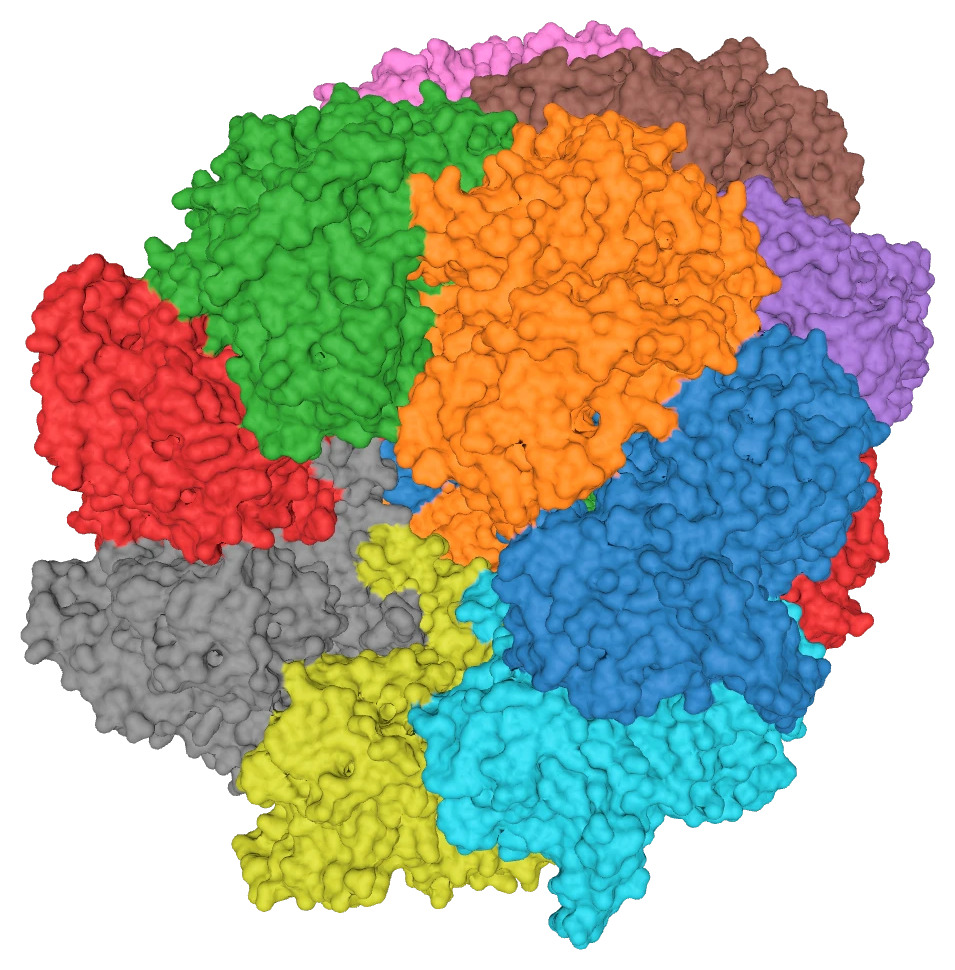
\includegraphics[width=\linewidth]{1aon-chain}
    \caption{1AON, by chain}
  \end{subfigure}\hfill
  \begin{subfigure}[b]{0.30\linewidth}
    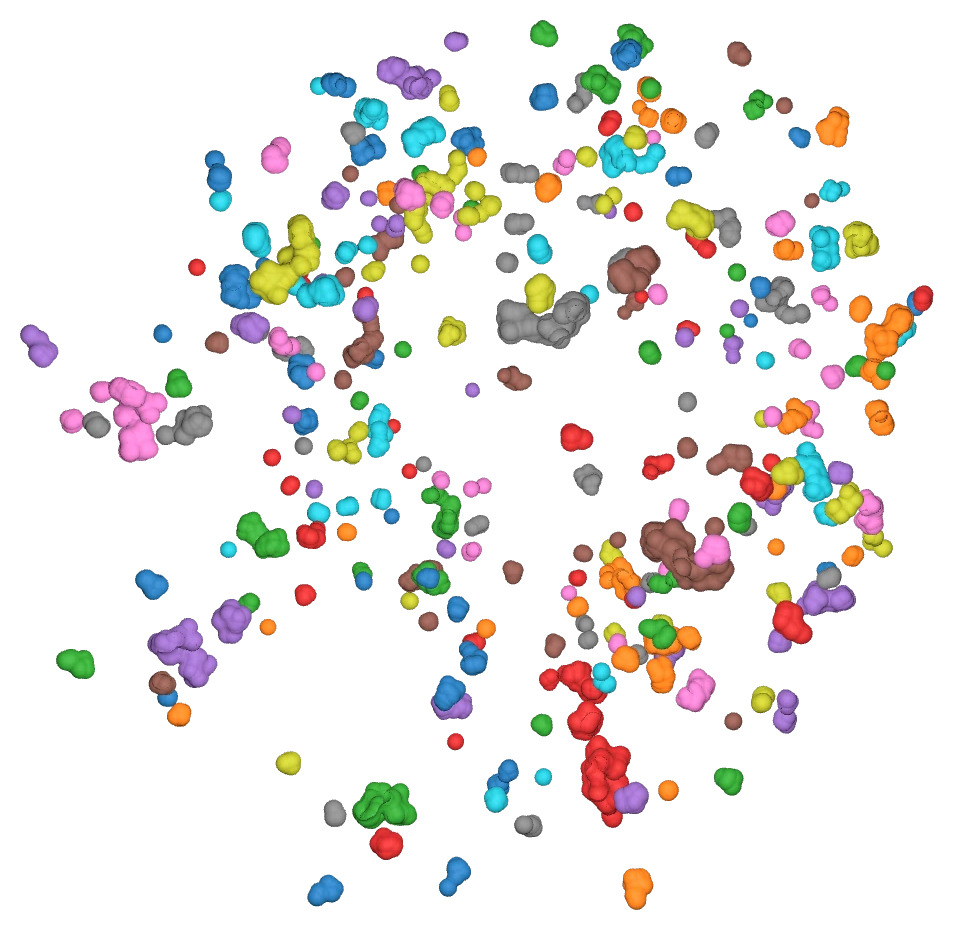
\includegraphics[width=\linewidth]{1aon-cavities}
    \caption{1AON cavities}
  \end{subfigure}\hfill
  \begin{subfigure}[b]{0.36\linewidth}
    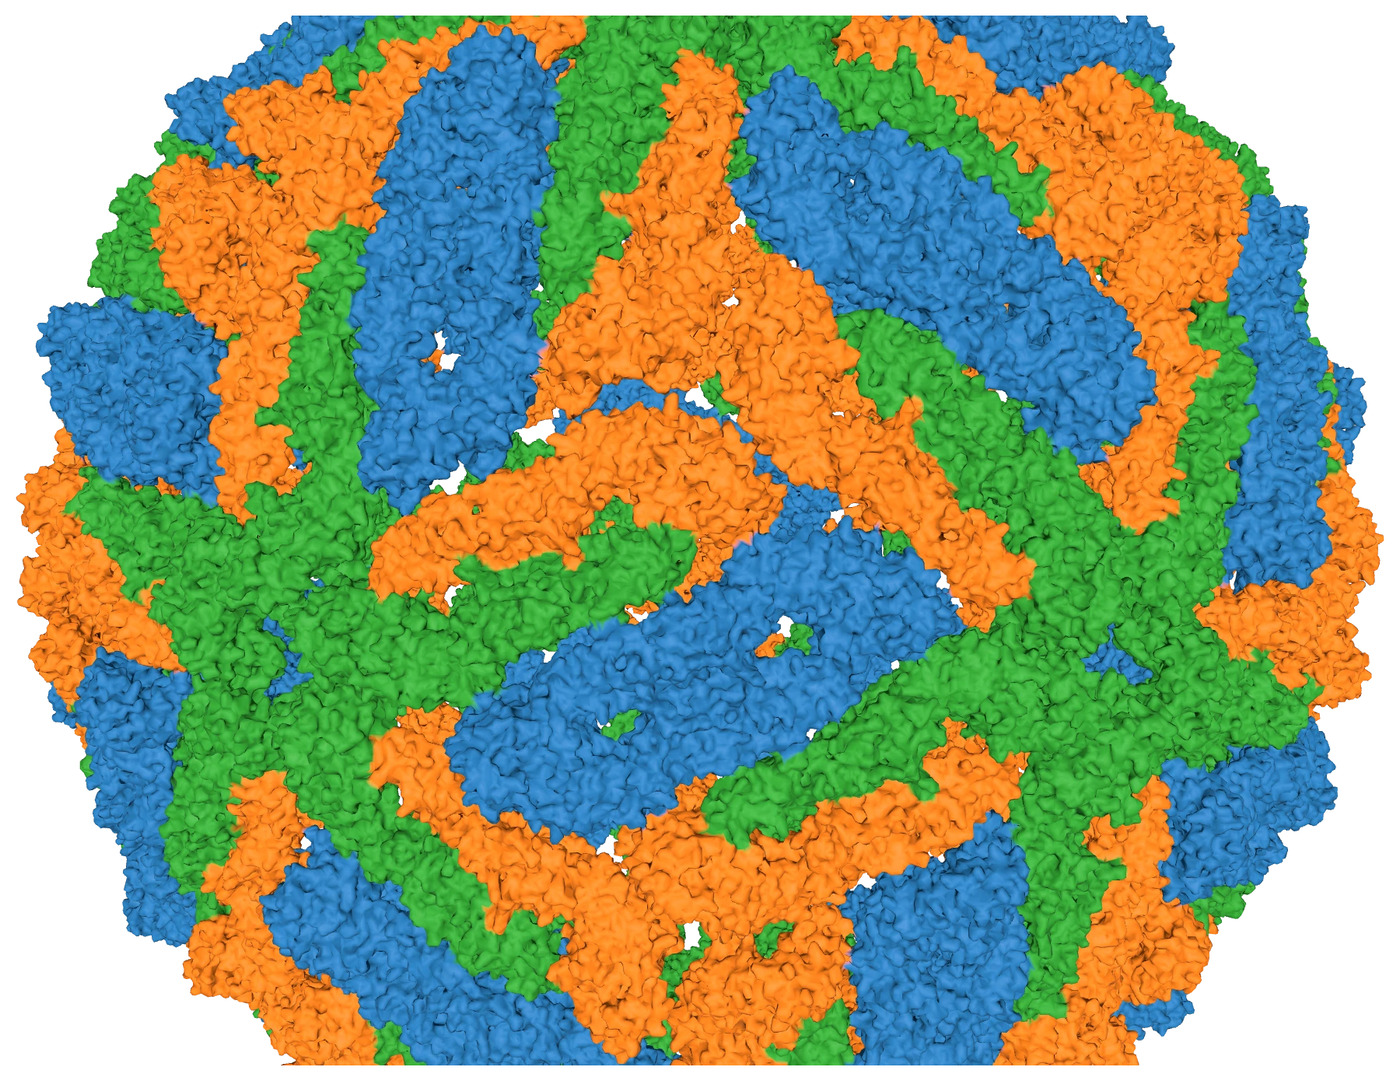
\includegraphics[width=\linewidth]{1k4r-capsid}
    \caption{1K4R capsid}
  \end{subfigure}
  \caption{(a)~GroEL--GroES (21 chains, 58\,870 atoms) at 0.5\Ang,
    decimated to 1.5\,M triangles. (b)~The same view showing only its 285
    internal cavities larger than 5\AA$^3$ (from a 0.25\Ang{} mesh), one
    colour each. (c)~Assembly~1 of the dengue virus capsid 1K4R, 60 copies
    of three envelope chains (545\,040 atoms) built from the file's
    operators, meshed at 1\Ang{} and decimated from 9.9\,M to 3\,M
    triangles for rendering.}
  \label{fig:gallery-large}
\end{figure}
